\documentclass{article}

% if you need to pass options to natbib, use, e.g.:
%     \PassOptionsToPackage{numbers, compress}{natbib}
% before loading neurips_2021

% ready for submission
\usepackage{neurips_2021}

% to compile a preprint version, e.g., for submission to arXiv, add add the
% [preprint] option:
%     \usepackage[preprint]{neurips_2021}

% to compile a camera-ready version, add the [final] option, e.g.:
%     \usepackage[final]{neurips_2021}

% to avoid loading the natbib package, add option nonatbib:
%    \usepackage[nonatbib]{neurips_2021}

\usepackage[utf8]{inputenc} % allow utf-8 input
\usepackage[T1]{fontenc}    % use 8-bit T1 fonts
\usepackage{hyperref}       % hyperlinks
\usepackage{url}            % simple URL typesetting
\usepackage{booktabs}       % professional-quality tables
\usepackage{amsfonts}       % blackboard math symbols
\usepackage{nicefrac}       % compact symbols for 1/2, etc.
\usepackage{microtype}      % microtypography
\usepackage{xcolor}         % colors



\usepackage{amsmath, amsfonts, amsthm}
\usepackage{enumerate}
\usepackage{graphicx}
\usepackage{subcaption}

\theoremstyle{definition}
\newtheorem*{definition}{Definition}
\newtheorem{theorem}{Theorem}
\newtheorem{corollary}{Corollary}
\newtheorem{assumption}{Assumption}
\newtheorem*{remark}{Remark}

\newcommand{\ah}[1]{\textcolor{blue}{AH: \textit{#1}}}
\newcommand{\fb}[1]{\textcolor{red}{FB: \textit{#1}}}

\newcommand{\agentset}{\mathcal{N}}
\newcommand{\edgeset}{\mathcal{E}}
\newcommand{\weightset}{W}

\newcommand{\actionset}[1]{S^{#1}}
\newcommand{\utility}[1]{u^{#1}}

\newcommand{\wmunu}{w^{\mu \nu}}
\newcommand{\xmu}{x^{\mu}}
\newcommand{\xnu}{x^{\nu}}
\newcommand{\refmu}{\sigma^{\mu}}
\newcommand{\avgref}[1]{\alpha_\sigma^{#1}}
\newcommand{\NE}[1]{\bar{x}^{#1}}
\newcommand{\weightedsum}{ \sum_{\nu \in N^\mu} \wmunu \xnu}
\newcommand{\xnotmu}{x^{-\mu}}
\newcommand{\xmuaction}[1]{x^{\mu}_{#1}}

\newcommand{\pure}[2]{e^{#1}_{#2}}


\title{Fictitious Play in Network Aggregative Games}

% The \author macro works with any number of authors. There are two commands
% used to separate the names and addresses of multiple authors: \And and \AND.
%
% Using \And between authors leaves it to LaTeX to determine where to break the
% lines. Using \AND forces a line break at that point. So, if LaTeX puts 3 of 4
% authors names on the first line, and the last on the second line, try using
% \AND instead of \And before the third author name.

\author{%
 Aamal Hussain  \\
  Department of Computing\\
  Imperial College London\\
  South Kensington, London \\
  \texttt{aamal.hussain15@imperial.ac.uk} \\
  % examples of more authors
  \And
  Francesco Belardinelli
  % Coauthor \\
  % Affiliation \\
  % Address \\
  % \texttt{email} \\
  % \AND
  % Coauthor \\
  % Affiliation \\
  % Address \\
  % \texttt{email} \\
  % \And
  % Coauthor \\
  % Affiliation \\
  % Address \\
  % \texttt{email} \\
  % \And
  % Coauthor \\
  % Affiliation \\
  % Address \\
  % \texttt{email} \\
}

\begin{document}

\maketitle

\begin{abstract}
  The abstract paragraph should be indented \nicefrac{1}{2}~inch (3~picas) on
  both the left- and right-hand margins. Use 10~point type, with a vertical
  spacing (leading) of 11~points.  The word \textbf{Abstract} must be centered,
  bold, and in point size 12. Two line spaces precede the abstract. The abstract
  must be limited to one paragraph.
\end{abstract}

\section{Introduction}

Multi Agent Learning \cite{Schwartz} requires a number of agents to adapt in an environment where
each agent must adapt in response to the behaviour of the other agents. This leads to a
fundamentally non-stationary problem, which presents a challenge to designing effective learning
policies. Even when there are a small number of agents in the game, learning has been shown to lead
to non-stationary, and even chaotic behaviour \cite{SatoChaos}, and this problem becomes even more
pronounced as the number of agents increase \cite{Sanders}. In this light, it would appear that
learning when there is a large population of agents is an impossible task. 

To deal with this problem, one must attempt to reduce the many player game to something which is
tractable. A number of reductions have been proposed, most notably \emph{Mean Field} Games
and \emph{Aggregative} Games. The former makes the assumption of an infinite
number of agents, so that the population can be represented through a distribution over players'
states \cite{CainesPaper} . Every agent then updates their action profiles depending on this
distribution. In the latter each agent plays considers a real valued function which is a convex
combination of the states of the other agents. In both formulations, a many player game is reduced
to the set of two player games which each agent is involved in, allowing the problem to maintain
tractability. 

Whilst both formulations have shown success in multi-agent learning settings, allowing agents to
reach equilibrium strategies (c.f. \cite{MFGLearningPapers} for Mean Field Games and
\cite{Aggregative Papers} for Aggregative Games), they also present a fundamental limitation.
Namely, they both require that agents have access to the action profiles of the entire population.
This could be through communication with all other agents, or through the intervention of a central
coordinator who is able to the entire population. Whilst recent work aims to relax this assumption
through the introduction of noise \cite{MFG-FP} or partial observability \cite{AAMASPaper}, the
requirement that each agent updates their actions based on the entire population is rather strong.

In this study, we investigate a variant of the aggregative game known as the \emph{Network
Aggregative} (NA) Game. This format assumes that there is an underlying communication network
through which agents interact. Then each agent updates their actions according only to those agents
with whom they communicate. This significantly relaxes the communication load on each agent and
lifts the need for a central coordinator. Recent work on the NA game has shown that it is possible
for agents to reach an equilibrium strategy in an entirely distributed manner \cite{Grammatico,
LeaderFollower, MyopicAgents}. We contribute in this direction by showing that learning on an NA
game can lead to an equilibrium strategy. In particular, we analyse the Fictitious Play Learning
Algorithm \cite{Brown, Harris}, in which agents are assumed to be myopic, in that they react solely
to the previous behaviour of the others.


\subsection{Contributions}

  The main contribution of this work is to study the behaviour of the Fictitious Play (FP) learning
  algorithm, in continuous time, when applied on a Network Aggregative Matrix Game.


  We first show that a Nash Equilibrium exists and that FP admits
  solutions in this setting. In particular, we study zero-sum games and show that
  Fictitious Play converges to a fixed point, which for a network without any
  self-loops corresponds to a Nash Equilibrium. In addition, we find that, for games
  which are not zero-sum, agents following Fictitious Play are able to
  achieve no regret.

  Finally, we explore FP through numerical simulations to consider the
  question of whether it always converges. We answer this in the negative by finding a family of
  games in which action profiles cycle around the Nash Equilibrium. Finally, our experiments
  document how noise affects the convergence of Fictitious Play. Our experiments suggest that, under
  the presence of noise, the algorithm still reaches a fixed point, but perhaps not the Nash
  Equilibrium. This presents an interesting avenue for future research.

\subsection{Related Work}

\paragraph{Network Aggregative Games}

The NA game is a recent introduction \cite{Parise2015} which presents a variant of aggregative games
by adding an underlying structure to the population. Since its introduction, distributed algorithms
have been built with the aim of finding NE. In particular, \cite{Parise2015, Parise2020} consider
the case in which payoffs are given by Lipschitz functions with unique minimisers and apply standard
topological fixed point towards designing algorithms which will converge to the NE. We note that the
\emph{Mann Iteration}, one of the algorithms applied in \cite{Parise2020} shares a remarkably
similar form with the discrete variant of FP. To the best of our knowledge, this link has not been
explored in the literature and is an avenue for research which we are currently pursuing. Another
common algorithm for distributed NE seeking is the projected gradient (resp. subgradient) dynamics
which is explored in \cite{Zhang2020} (resp. \cite{Shokri2020, Shokri2021}). In all of these works,
the cost function is assumed to be convex, and therefore have a unique minimiser. In fact this is a
common assumption in works concerning NA Games \cite{Zhu2021, Lei2020}, which we believe is due to
its ubiquity in control settings. We have not yet come across works which consider NA games from the
point of view of payoff matrices, which are more common in multi agent learning settings.
Furthermore, to the best of our knowledge, this is the first work which introduces the application
of a strict learning algorithm in the NA setting.

\paragraph{Fictitious Play}

Fictitious Play was introduced by Brown in 1951 \cite{BrownPublished, BrownUnpublished} as a
'natural' way in which to approximate the Nash Equilibrium in zero sum games. It was known at the
time that a discrete variant of the algorithm would converge to the NE in two player zero-sum games
\cite{Robinson}. Since then a number of proofs of convergence were determined in 2 player games
\cite{Miyasawa, Polak, Berger, Monderer and Sela, Monderer and Shapley}, as well as corresponding
convergence rates \cite{Harris, Shapiro}. Many results hold for both the discrete and continuous
variants of FP. Their relation was finally solved by Hofbauer \cite{Hofbauer}, who showed that
attractors of the discrete time process are also attractors for the continuous time variant. As
such, most of the analysis on FP focuses on the continuous time variant \cite{Ostrovski}. It was
later shown in \cite{Shapley} that there is a family of games (now called the \emph{Shapley family})
for which FP does not converge at all but rather shows periodic behaviour. This led to research
which looks at this non convergent behaviour, specifically showing the existence of more periodic
orbits as well as chaotic behaviour \cite{Sparrow}. However, the work looking at fictitious play
where there are more than two agents is sparse. \cite{Sela} considers a game in which a multi-player
game is decomposed by requiring that each agent engage in a two person game against each of the
opponent. Their payoff is given by the sum of payoffs in all of these subgames. It was found that,
if this game is zero sum, then FP will converge. Similar results for more than two players were
found for games with identical interests in \cite{MondererShapley1994}. In \cite{FPMFG}, the action
of FP was considered in a Mean Field Game, and it was found again that the algorithm converges for
zero sum games. The most general result, and the one most similar to our own, was found by Ewerhart
and Valkanova in 2020 \cite{Ewerhart} in which they showed that fictitious play converges in network
games, where each agent is engaged in a two-player game with each of their neighbours. The rate of
convergence was found to be independent of the network size.  Our work extends the analysis of FP in
multiplayer games by considering its action in NA Games, so that the agents do not play individual
games against each of their neighbours but rather a single game against the aggregate of their
neighbours. In particular we also extend a result for two player games found by Ostrovski and van
Strein \cite{Payoff Performance} which showed that FP achieves no-regret to the multi-player
setting.

\section{Preliminaries}
\subsection{Network Aggregative Games}
\label{sec::NAG}

  The model we consider is that there is a set $\agentset = {1,
           \ldots , N}$ of agents who are connected through an underlying
          interaction graph. This graph is given by the tuple
          $(\agentset, (\edgeset, \weightset))$ in which $\edgeset$ is
          the set of all pairs $(\mu, \nu) \in \agentset \times \agentset$
          connected. Formally,
        
  \begin{definition}[Interaction Graph]
    Given a set $\agentset$ of agents, an {\em interaction graph} $I = (\agentset, (\edgeset,
    \weightset))$ such that
    \begin{itemize}
    \item $\edgeset \subseteq \agentset \times \agentset$.        Then, the set of neighbours of agent
        $\mu$ is denoted as $N^\mu = \{\nu \in \agentset \, : \, (\mu, \nu) \in \edgeset\}$.
      \item $\weightset \in M_N(\mathbb{R})$ is the weighted adjacency matrix whose elements $w^{\mu
        \nu}$ expresses the importance that agent $\mu$ places on agent $\nu$. If $(\mu, \nu) \not
        \in \edgeset$ then $w^{\mu \nu} = 0$;        $\wmunu \in (0, 1]$ otherwise.
    \end{itemize}
  \end{definition}

  With the above definition, we can formalise the network aggregative (NA) game:

  \begin{definition}[Network Aggregative Game]
    A Network Aggregative game is defined as the tuple $\Gamma = (I, (\actionset{\mu},
        \utility{\mu})_{\mu \in \mathcal{N}})$, where $I$ is the interaction graph,
        $\actionset{\mu}$ and $\utility{\mu}$ refer to $\mu$'s set of actions (with cardinality
        $|\actionset{\mu}| = n$) and utility function respectively.
  \end{definition}

  We consider the \emph{state} of agent $\mu$ to be the probability vector $\xmu \in
  \mathbb{R}^n$ where $\xmu_i$ is the probability with which the agent plays action $i$. It
  should be noted that this probability vector is often referred to as $\mu$'s \emph{mixed
  strategy}. With this in mind, we can construct, as their state space, the unit simplex on
  agent $\mu$'s action set. This is given as $\Delta_\mu := \{\xmu \in \mathbb{R}^n \, : \,
  \sum_i \xmuaction{i} = 1\}$. Also associated with each agent is a utility function

  The utility function, for each agent $\mu$, is given as $u^\mu(\xmu, \xnotmu)$ in which we use
  the standard notation $-\mu$ to refer to all agents other than $\mu$. Notice that this requires
  that each agent play the same strategy against all of their neighbours. What is unique about the
  NA game is the structure of the payoffs themselves. In this format, each agent is receives a
  reference $\sigma$ which is a weighted sum of each of their neighbours
  state. Formally
  %
  \begin{equation}
    \sigma^\mu = \sum_{\nu \in N^\mu} \wmunu \xnu.
  \end{equation}

  Then, the agent's must optimise their payoff with respect to this reference vector. Thus,
  instead of having to consider the actions of the entire population, or play individual games
  against each of their neighbours, the agent only has to consider $\sigma^\mu$ as a
  `measurement' of the local aggregate state and optimise with respect to this measurement.
  This allows us to make the reduction $u^\mu(\xmu, \xnotmu) = u^\mu(\xmu, \refmu)$. In
  particular, we consider that the agent is engaged in a matrix game against the
  reference vector so that
  %
  \begin{equation}
    u^\mu(\xmu, \refmu) = \xmu \cdot A^\mu \refmu = \xmu
                \cdot A^\mu \weightedsum.
  \end{equation}

  where $A^\mu$ is the payoff matrix associated to agent $\mu$. Note that this means we can write
  the game $\Gamma$ with the payoff matrices $A^mu$ in place of the utility functions
  $\utility{\mu}$. The NA game allows for the reduction of a multiplayer game into a series of
  two-player games. The agent's goal is to maximise their payoff with respect to the reference
  vector. As such, we define the best response correspondence $BR^\mu$ which maps any $\refmu$
  the set $\arg \max_{y \in \Delta_\mu} {u^\mu(y, \refmu)}$. 

  Finally, a central concept of game theory is that of the Nash Equilibrium, in which no rational
  agent has the incentive to deviate from their current state. This can be formalised by saying
  that all agents are playing the best response to each other.

  This leads naturally to the definition of a Nash Equilibrium in an NA Game as

  \begin{definition}(NE)
    The set of vectors $\{ \NE{\mu}\}_{\mu \in \agentset}$ is an NE if, for all $\mu$,  
    \begin{equation*}
    \NE{\mu} \in BR^\mu (\refmu) = \arg \max_{x \in \Delta_\mu} u^\mu(x, w^{\mu \mu} x + \sum_{\nu \in N^\mu \backslash \{\bar{\mu}\}} \wmunu \NE{\nu}).
    \end{equation*} 
  \end{definition}
    
  \begin{remark}
    It can be seen that the concept of the Nash Equilibrium in the NA game is a natural
    extension of the NE in a bimatrix game $(A, B)$. In particular, if we consider an NA game
    with only two players and no self-loops then the above definition yields

    \begin{equation*}
      \NE{1} \in BR^1 (\sigma^1) = \arg \max_{x in \Delta_1} u^1 (x, \NE{2}), 
    \end{equation*}

    and similarly for $\NE{2}$. This is precisely the definition of an NE in a two player game \cite{}.
  \end{remark}

  We will show that the NE exists for an NA game in Section \ref{sec::ExistenceofNE}. 

  Finally we note that an NA game is \emph{zero-sum} if the utilities of each agent sum to zero for any strategy set $\{ \xmu \}_{\mu \in \agentset}$. Formally

  \begin{equation}
    \sum_\mu u^\mu(\xmu, \weightedsum) = 0.
  \end{equation}

\subsection{Continuous Time Fictitious Play}
\label{sec::CTFP}

  Fictitious Play requires that, at the current time, each agent considers the average state
  of their opponent in the past, and respond optimally (i.e. play a best response) to this state. In the case of an NA game, each agent considers their reference vector to be their
  opponent. As such, each agent $\mu$ must update their state according to the time-average of
  $\refmu$. To formalise this we write

  \begin{equation}
    \avgref{\mu} = \frac{1}{t} \int_0^t \refmu(s) \; ds.
  \end{equation}

  Using this, we follow in the footsteps of Ewerhart \cite{} and Harris \cite{} to define
  Fictitious Play in continuous time.
%
  \begin{definition}[Continuous Time Fictitious Play (CTFP)]
    A CTFP is defined as a measurable map $m$ with components $m^\mu$ such that for all $\mu$
    and all $t \geq 1$, $m^\mu: [0, \infty) \rightarrow \Delta_\mu$ satisfies $m^\mu(t) \in
    BR^\mu(\alpha_{\sigma}^\mu)$ for almost all $t \geq 1$.
  \end{definition}

  We can think of this definition as saying that the player plays some arbitrary strategy before
  $t = 1$, but beyond this it must play a best response to the time average of its reference
  signal.
  
  \begin{remark}
    As an illustration, consider the NA game with two players, in which $\edgeset = \{(1, 2),
    (2, 1)\}$ and $\weightset$ is a 2x2 matrix with zeros on its leading diagonal and ones on
    the off diagonal. We write the time-average of both agents' state as
  
    \begin{align}
      \alpha^\mu = \frac{1}{t} \int_0^T \xmu(t) \, dt & \text{ for $\mu \in \{1, 2\}$}
  %   \alpha^2 = \frac{1}{t} \int_0^T x^2(t) \, dt \\
    \end{align}

    In this manner, the $\alpha^\mu(t)$ denotes the time average of the strategies played by
    agent $\mu$ up to time $t$. Then, fictitious play requires that the agents update their
    strategy as $x^1(t) \in BR^1(\alpha^2(t))$ and $x^2(t) \in BR^2(\alpha^1(t))$. It can be
    seen, therefore, that the CTFP in an NA game is a natural extension of CTFP in the classical
    two-player setting \cite{}.
  \end{remark}

\subsection{Assumptions}

  With the above preliminaries in place, we can state the assumptions that we make in this study.

  \begin{assumption}
    The weighted adjacency matrix $\weightset$ is constant and \emph{row stochastic} meaning
    that the sum elements in each row of $\weightset$ is equal to one. This assumption is
    made to ensure that the analysis of NA games can be derived as a natural extension to the
    classical setting of two-player games. We can think of the row stochastic condition as the
    ability of each agent to prioritise the state information it receives from each of its
    neighbours. It is also a classical assumption made in the analysis of network games
    \cite{one of the network game papers} and can is straightforward to implement \cite{Eyad}.
  \end{assumption}

  \begin{assumption}
    The payoffs are given through matrix games and, therefore, are bilinear. Payoff matrices
    have a rich history in game theory and has generated a number of prototypical examples for
    economic study including the Prisoner's Dilemma game (see \cite{Axelrod} for an interesting
    implementation of this). They also allow for the design of multi-agent systems in
    computational settings, particularly in the case of task and resource allocation \cite{AGT
    and some of the Applied Game Theory Papers}. It should be noted, however, that game
    theoretic analysis is starting to consider various other forms of utility functions,
    including monotone \cite{Maryam} and convex \cite{Parise}. We believe that the analysis of
    Fictitious Play should follow in these developments and we consider it as an important area
    of future work.
  \end{assumption}

  \begin{assumption}
    The cardinality of each action set $|\actionset{\mu}|$ is equal for all agents. This is
    a classical assumption which is made in most game theoretic settings and includes, as a
    special case, the analysis of homogeneous agents \cite{}. However, it should be noted that,
    in \cite{Ewerhart}, CTFP was analysed without this requirement.  
  \end{assumption}

  \begin{assumption}
    The NA game is zero-sum in the sense that $\sum_{\mu} u^\mu(\xmu, \weightedsum)$ for any set
    of states $(x^\mu)_{\mu \in N^\mu}$. This is, perhaps, one of the stronger assumptions in
    our analysis, and is required for the fixed point analysis. However, in Section
    \ref{sec::CCEConvergence}, we perform a regret analysis that considers the long term
    behaviour of CTFP without this assumption.
  \end{assumption}

\section{Convergence of Fictitious Play}

  \subsection{Existence of the Nash Equilibrium}
  \label{sec::ExistenceofNE}
  
  Note that the NE Condition requires

  \begin{align}
    \NE{\mu} &\in \arg\max_{x \in \Delta_\mu} u^\mu(x, w^{\mu \mu}x + \sum_{\nu \in N^\mu} w^{\mu \nu} \NE{\nu}) \nonumber \\
    & =: \arg\max_{x \in \Delta_i} \bar{u}^\mu(x, \sum_{\nu \in N^\mu} w^{\mu \nu} \NE{\nu})
  \end{align}

  where we can find $\bar{u}_i$ through the following argument
  
  \begin{align}
    u^\mu(x, w^{\mu \mu} x + \sum_{\nu \in N^\nu} w_{\mu \nu} \NE{\nu}) & = x \cdot A^\mu (w^{\mu \mu} x + \sum_{\nu \in N^\mu} w_{\mu \nu} \NE{\nu}) \\
     & = x \cdot (w^{\mu \mu} A^\mu)  x + \sum_{\nu \in N^\mu} u^{\mu \nu}(x, \NE{\nu}) \\
     & =: \bar{u}^\mu(x, \sum_{\nu \in N^\mu} w^{\mu \nu} \NE{\nu}), \nonumber
  \end{align}
  
  where $u^{\mu \nu}(\xmu, x^\nu) = \xmu \cdot A^\mu x^\nu$. Note that, in order to get this
  formulation, we had to use the assumption of payoffs being bilinear so that we could separate
  out the term in the weighted sum involving $x$ from $\bar{x}^\nu$. 
  
  To show existence of an NE we will need the following definition and theorem.

  \begin{definition}[Upper Semi-Continuous]
    A compact-valued correspondence $\Phi: A \rightarrow B$ is \emph{upper semi-continuous} at a point $a$ if $g(a)$ is non-empty and if, for every sequence $a_n \rightarrow a$ and every sequence $(b_n)$ such that $b_n \in g(a_n)$ for all $n$, there exists a convergent subsequence of $(b_n)$ whose limit point $b$ is in $g(a)$.  
  \end{definition}

  \begin{theorem}[Kakutani]
    Let $K \subset \mathbb{R}^n$ be compact and convex and $\Phi: K \rightarrow K$ be closed or upper semi-continuous, with nonempty, convex and compact values. Then $\Phi$ has a fixed point.
  \end{theorem}

  Note that, when acting on a simplex, the function $\Phi: \Delta \rightarrow \textbf{P}(\Delta)$, where $\textbf{P}(\Delta)$ denotes the nonempty, closed and convex subsets of $\Delta$ only has to satisfy the upper-semi continuity condition to admit a fixed point.

  \begin{theorem}[Existence of NE]
    Under the assumption (II), namely that the payoff function achieves a bilinear property, a
    Nash Equilibrium $\{\bar{x}^\mu\}_{\mu \in \agentset}$ exists.
  \end{theorem}

  \begin{proof}
    We begin by rewriting the NE condition by concatenating the set of NE vectors into one long colunn vector. This gives

    \begin{equation}
      \begin{bmatrix}
        \bar{x}^1 \\ . \\ . \\ . \\ \bar{x}^N
      \end{bmatrix} \in
      \begin{bmatrix}
      \arg\max_{y \in \Delta_1} \bar{u}^1(y, \sum_{\nu \in N^1} w^{1 \nu} \bar{x}^\nu) \\ . \\ . \\ . \\ \arg\max_{y \in \Delta_N} \bar{u}^1(y, \sum_{\nu \in N^N} w^{N \nu} \bar{x}^\nu)
      \end{bmatrix} .
    \end{equation}

    We can rewrite the weighted summation for $\mu$ as

    \begin{equation}
      \sum_{\nu \in N^\mu} w^{\mu \nu} \bar{x}^\nu = (w_{-\mu}^T \otimes I_n) \begin{bmatrix}
        \bar{x}^1 \\ . \\ . \\ . \\ \bar{x}^N
      \end{bmatrix},
    \end{equation}
  
    in which $w_{-\mu}$ is a column vector containing $w^{\mu \nu}$ in the $\nu$'th element for all $j \in N^\mu$ and 0 everywhere else (including in the $\mu$'th slot), $I_n$ is the $n \times n$ identity matrix and $\otimes$ is the kronecker product. For example, the form for agent 1, in the case of 2-action game is given by

    \begin{equation}
      (w_{-1}^T \otimes I_2) = [0, w_{12}, w_{13}, ..., w_{1n}] \otimes I_2 = 
      \begin{bmatrix}
        0 & 0 & w_{12} & 0 & ... & w_{1n} & 0 \\
        0 & 0 & 0 & w_{12} & ... & 0 & w_{1n} \\
      \end{bmatrix}
    \end{equation}
    
    Returning to the $N$-player NA game our condition becomes
    \begin{equation}
      \begin{bmatrix}
        \NE{1} \\ . \\ . \\ . \\ \bar{N}
      \end{bmatrix} \in
      \begin{bmatrix}
        \arg\max_{y \in \Delta_1} \bar{u}^1(y, (w_{-1}^T \otimes I_n) \begin{bmatrix}
          \NE{1} \\ . \\ . \\ . \\ \NE{N}
        \end{bmatrix}) \\ . \\ . \\ . \\ \arg\max_{y \in \Delta_N} \bar{u}_N(y, (w_{-N}^T \otimes I_n) \begin{bmatrix}
        \NE{1} \\ . \\ . \\ . \\ \NE{N}
      \end{bmatrix}))
      \end{bmatrix} .
    \end{equation}

    This means that we achieve a Nash Equilibrium iff $(\NE{\mu})_{\mu \in \agentset}$ is a fixed point of the map
  
  
    \begin{equation}
      \begin{bmatrix}
        \arg\max_{y \in \Delta_1} \bar{u}^1(y, (w_{-1}^T \otimes I_n) ( \cdot )) \\ . \\ . \\ . \\ \arg\max_{y \in \Delta_N} \bar{u}^N(y, (w_{-N}^T \otimes I_n)( \cdot ))
      \end{bmatrix} .
    \end{equation}


    Now, since the modified payoff $\bar{u}^\mu$ shares the same bilinear property as $u^\mu$, we can assert that it is continuous is its second argument. Therefore, the above vector valued map can be asserted to be continuous and so is upper semi-continuous. As such, we can apply Kakutani's Fixed Point Theorem to assert that the above map admits a fixed point.

  \end{proof}

\subsection{Existence of CTFP}

  \begin{theorem}
    There exists a path $m$ which satisfies the property that, for all $\mu$, $m^\mu \in
    BR^\mu(\alpha_\sigma^\mu)$ for almost aall $t \geq 1$.
  \end{theorem}

  \begin{proof}
    Recall the definition of $\alpha^\mu(t)$

    \begin{equation*}
    \alpha^\mu(t) = \frac{1}{t} \int_{0}^{t} m^\mu(s) \, ds
    \end{equation*}

    Then 

    \begin{align}
    \frac{d}{dt} \alpha^\mu(t) & = \frac{d}{dt} \frac{1}{t} \int_{0}^t m^\mu(s) ds \nonumber \\
    & = \frac{1}{t} m^\mu(t) - \frac{1}{t} \alpha^\mu(t)
    \end{align}

    Now we assert that $m^\mu(t) \in BR^\mu(\alpha_{\sigma}^\mu) = \arg\max_{y \in \Delta_\mu} u^\mu(y,
    w^{\mu \mu} \alpha^\mu(t) + \sum_{\nu \in N^\mu} w_{ij} \alpha^\nu(t))$. 

    Let us then define $\alpha(t)$ as the concatenation of all $\alpha_i(t)$

    \begin{equation}
      \alpha(t) = \begin{bmatrix}
        \alpha^1(t)^T, \ldots, \alpha^N(t)^T
      \end{bmatrix}^T \subset \mathbb{R}^{Nn}
    \end{equation}


    We can, therefore, write the aggregation as

    \begin{equation}
      (W \otimes I_n) \alpha(t) = \begin{bmatrix}
        \sum_{\nu \in N^1} w^{1 \nu} \alpha^\nu(t) \\
        .\\
        .\\
        .\\
        \sum_{\nu \in N^N} w^{N \nu} \alpha^\nu(t)
      \end{bmatrix} \subset \mathbb{R}^{Nn}
    \end{equation}

    I will write $(W \otimes I_n) \alpha(t)$ as $\alpha_W$ for convenience. Furthermore, using
    the bilinear property of the game, we can say that

    \begin{equation}
      \begin{bmatrix}
        \arg\max_{y_1 \in \Delta_1} y \cdot A^1 ( \alpha_W(t))_1 \\
        .\\
        .\\
        .\\
        \arg \max_{y_N \in \Delta_N} y \cdot A^N (\alpha_W(t))_N 
      \end{bmatrix} = 
      \arg \max_{y \in \Delta} y \cdot \begin{bmatrix}
        A^1 & 0 & . & . & . & 0 \\
        0 & A^2 & . & . & . & 0 \\
        & & . & & & \\
        & & & . & & \\
        & & & & . & \\
        0 & 0 & . & . & . & A^N \\
      \end{bmatrix} \alpha_W(t) = \arg\max_{y \in \Delta} y \cdot \Lambda (W \otimes I_n)
      \alpha(t)
    \end{equation}

    in which $\Delta = \times_i \Delta_i$ and $\Lambda$ is the block diagonal matrix containing
    each $A^i$. 

    We can now write the differential inclusion as

    \begin{equation}
      \dot{\alpha}(t) \in \frac{1}{t} (\arg \max_{y \in \Delta}  \{y \cdot \Lambda (W \otimes
      I_n)
      \alpha(t) \}- \alpha(t))
    \end{equation}

    with the initial condition $\alpha(1) = x_0$. Then, the path $m$ is a CTFP if its
    corresponding $\alpha(t; m)$ is a solution to the above differential inclusion. Following
    the definition of (Harris 1998), a solution $\alpha(t)$ must satisfy

    \begin{enumerate}
      \item $\alpha(t)$ is locally Lipschitz
      \item $\alpha(1) = x_0$
      \item $\dot{\alpha}(t) \in \frac{1}{t} (\arg \max_{y \in \Delta}  \{y \cdot \Lambda (W \otimes
      I_n)
      \alpha(t) \}- \alpha(t))$ for almost all $t \in [1, \infty)$ 
    \end{enumerate}

    The question then remains, does the differential inclusion admit a solution? Using the
    results of Aubin and Cellina (see Harris 1998, paragraph below Prop. 6), can use the fact
    that the $\arg \max$ function is non-empty, compact and convex valued, bounded (all of
    these follow since the function acts from $\Delta$ to $\Delta$) and upper semi-continuous. 
    With these facts in place, we can say that there is a CTFP $m$ for any initial value $x_0$. Further, the solution $m(t)$ is Lipschitz for almost all $t \geq 0$.

  \end{proof}

\subsection{Convergence of CTFP}

With the existence of the CTFP in place, we can show that it converges to a fixed point. In particular, let $\Omega(\alpha)$ be the set of all limit points for $\alpha(t)$. Then, a CTFP path is said to have converged if $\Omega(\alpha)$ is contained within the set of Nash Equilibria of the game. If this is for any such CTFP path, then the game is said to have the \emph{CTFP property}. We adapt the techniques of (Ewerhart 2020) to prove that zero-sum NA games have the CTFP property. \ah{I also want to attempt this with the techniques of Harris (which is quite similar) to see if it yields any new results}.

  \begin{theorem}
    Any zero-sum NA game has the property that, for any CTFP path $m$, the corresponding $\alpha(t; m)$ converges to a set of fixed points.
  \end{theorem}


  \begin{proof}

    \begin{equation}
      m^\mu(t) \in BR^\mu \left( \frac{1}{t} \int_{0}^{t} \sigma^\mu(s) ds \right).
    \end{equation}
    
    By the definition of Continuous Time Fictitious Play (CTFP) given by Ewerhart, we require that $m: [0, \infty) \rightarrow \times_\mu \Delta_\mu$ is a measurable mapping such that, for each $\mu$, $m^\mu(t) \in BR^\mu \left( \frac{1}{t} \int_{0}^{t} \sigma^\mu(t') dt' \right)$. Now notice,
    
    \begin{equation*}
      m^\mu(t) \in BR^\mu \left( \frac{1}{t} \int_{0}^{t} \sigma^\mu(t') dt' \right) \iff  \in x^\mu\in BR^\mu \left( \frac{1}{t} \int_{0}^{t} [w^{\mu \mu} m^\mu(s) + \sum_{\nu \in N^\mu} w^{\mu \nu} m^\nu(s)] \, ds \right)
    \end{equation*}
    
    Let us assume that $u^\mu$ takes the form $x \cdot A^\mu \sigma^\mu$ where $A^\mu$ is the payoff matrix associated with agent $\mu$. Then,
    
    \begin{align}
      & m^\mu \in \arg\max_{x \in \Delta^\mu} u^\mu(x,\frac{1}{t} \int_{0}^{t} [w^{\mu \mu} m^\mu(t') + \sum_{\nu \in N^\mu} w^{\mu \nu} m^\nu(s)] \, ds) \nonumber \\
      \iff & m^\mu \in \arg\max_{x \in \Delta_\mu} x \cdot A^\mu \left(\frac{1}{t} \int_{0}^{t} [w^{\mu \mu} m^\mu(t') + \sum_{\nu \in N^\mu} w^{\mu \nu} m^\nu(s)] \, ds \right) \nonumber \\
      \iff & m^\mu \in \arg \max_{x \in \Delta_\mu} x \cdot (w^{\mu \mu} A^\mu) \left( \frac{1}{t} \int_{0}^{t} m^\mu(s) ds\right) + \sum_{\nu \in N^\mu} x \cdot (\wmunu A^\nu) \left( \frac{1}{t} \int_{0}^{t} m^\nu(s) ds \right) \nonumber \\
      \iff & m^\mu \in \arg \max_{x \in \Delta_i} x \cdot A^{\mu \mu} \alpha^\mu(t; m) + \sum_{\nu \in N^\mu} x \cdot A^{\mu \nu} \alpha^\nu(t; m).
    \end{align}
    
    where each $A^{\mu \nu} = \wmunu A^\mu$ and $\alpha^\mu(t; m) =\frac{1}{t} \int_{0}^{t} m^\mu(s) ds$ as defined by Ewerhart. We can, therefore, think of the NA game as a network game in which each agent plays the same strategy against each of its neighbours, itself included. As such, any $m$ which satisfies the CTFP property for the equivalent network game also satisfies the CTFP requirement for the network aggregative game. 
    
    Continuing with this approach, let us look at the case where $\sum_\mu A^\mu =
    \textbf{0}_{n\times n}$ (i.e. a zero sum game). This means that $\sum_i u_i = 0$. Let
    $\xmu_\infty = \lim_{t \rightarrow \infty} \alpha^\mu(t; m)$. More specifically, $\xmu_\infty$
    belongs to the set of accumulation points of $\alpha^\mu(\cdot; m)$ (which is set valued since
    the $BR^\mu$ map is set valued). To say that the game has `converged' we require that every
    $\xmu_\infty = (x^1_\infty, ... x^N_\infty)$ is an NE. Under these conditions, we may adapt the
    techniques of (\cite{Ewerhart} Prop. 1) to show convergence.
    
    
    Let us take the Lyapunov function
    
    \begin{equation}
      L(x) = \sum_\mu \max_{y \in \Delta_\mu} \{u^\mu(y, w^{\mu \mu} \xmu + \sum_{\nu \in N^\mu} \wmunu \xnu) - u^\mu(\xmu, w^{\mu \mu} \xmu + \sum_{\nu \in N^\mu} \wmunu \xnu) \}
    \end{equation}
    
    Using the same transformation as before:
    
    \begin{align}
       u^mu(y, w^{\mu \mu} \xmu + \sum_{\nu \in N^\mu} w_{\mu \nu} \xnu) & =  y \cdot A^\mu (w^{\mu \mu} \xmu + \sum_{\nu \in N^\mu} \wmunu \xnu) \nonumber \\
       & =  y \cdot (w^{\mu \mu} A^\mu) \xmu + \sum_{\nu \in N^\mu} y \cdot (\wmunu A^\mu) \xnu \nonumber \\
        & =  \sum_{\nu \in N^\mu \cup \{\mu\}} y \cdot A^{\mu \nu} \xnu \nonumber 
    \end{align}
    
    Then,
    
    \begin{align}
    L(x) &= \sum_\mu \max_{y \in \Delta_\mu}\sum_{\nu \in N^\mu \cup \{\mu\}} y \cdot A^{\mu \nu} \xnu  - u^mu(\xmu, w^{\mu \mu} \xmu + \sum_{\nu \in N^\mu} w^{\mu \nu} \xnu) \} \nonumber \\
    &= \sum_\mu \max_{y \in \Delta_\mu} \{\sum_{\nu \in N^\mu \cup \{\mu\}} y \cdot A^{\mu \nu} \xnu  \} - \sum_\mu  u^\mu(\xmu, w^{\mu \mu} \xmu + \sum_{\nu \in N^\mu} w^{\mu \nu} \xnu) \nonumber \\
    &= \sum_\mu \max_{y \in \Delta_\mu} \{\sum_{\nu \in N^\mu \cup \{\mu\}} y \cdot A^{\mu \nu} \xnu  \} \nonumber 
    \end{align}
    
    where the last equality holds because $\sum_\mu u^\mu = 0$. Now, in parallel with (Ewerhart 2020) we recall that we defined $m^\mu(t)$ as the best response to $\alpha(t)$. As such,

    \begin{align}
      L(\alpha(t)) & = \sum_\mu \sum_{\nu \in N^\mu \cup \{\mu\}} m^\mu(t) \cdot A^{\mu \nu} \alpha^\nu(t) \\
      t L(\alpha(t)) & = \sum_\mu \sum_{\nu \in N^\mu \cup \{\mu\}} m^\mu(t) \cdot A^{\mu \nu} t \alpha^\nu(t) \\
      t L(\alpha(t)) & = \sum_\mu \sum_{\nu \in N^\mu \cup \{\mu\}} m^\mu(t) \cdot A^{\mu \nu} \int_0^t m^\nu(s) ds
    \end{align}

    Similarly, since we know that $m^\mu(t')$ is a best response to $\alpha(t')$ at time $t'$ we have

    \begin{align}
      \sum_{\nu \in N^\mu \cup \{\mu\}} m^\mu(t') \cdot A^{\mu \nu} \alpha^\nu(t') & \geq \sum_{\nu \in N^\mu \cup \{\mu\}} m^\mu(t) \cdot A^{\mu \nu} \alpha^\nu(t') \\
      t' \sum_\mu \sum_{\nu \in N^\mu \cup \{\mu\}} m^\mu(t') \cdot A^{\mu \nu} \alpha^\nu(t') & \geq \sum_\mu \sum_{\nu \in N^\mu \cup \{\mu\}} m^\mu(t) \cdot A^{\mu \nu} \int_0^{t'} m^\nu(s) ds \\
      t' L(\alpha(t')) & \geq \sum_\mu \sum_{\nu \in N^\mu \cup \{\mu\}} m^\mu(t) \cdot A^{\mu \nu} \int_0^{t'} m^\nu(s) ds 
    \end{align}

    Combining the above equations in $t L(\alpha(t))$ and $t' L(\alpha(t'))$, we get

    \begin{align}
      t L(\alpha(t)) - t' L(\alpha(t')) \leq \sum_\mu \sum_{\nu \in N^\mu \cup \{\mu\}} m^\mu(t) \cdot A^{\mu \nu} \int_{t'}^{t} m^\nu(s) ds 
    \end{align}

    We can divide this expression by $t - t'$ and take the limit for $t' \rightarrow t$. This yields the derivative (in particular the upper right Dini derivative)

    \begin{equation}
      \limsup_{t' \rightarrow t, t' < t}\frac{t L(\alpha(t)) - t' L(\alpha(t'))}{t - t'} \leq 0
    \end{equation}

    As this derivative is (weakly) negative, and we know that $tL(\alpha(t))$ is continuous in $t$, we have the result that $t L(\alpha(t))$ is monotone decreasing. Therefore, it is bounded, i.e. there is some $C \geq 0$ such that $L(\alpha(t)) \leq C/t$. In addition, we know that each term in the summation in the original expression of the Lyapunov function is non-negative and so we can say that

    \begin{align}
      & \max_{y \in \Delta_\mu} \{u^\mu(y, w^{\mu \mu} \xmu + \sum_{\nu \in N^\mu} \wmunu \xnu) - u^\mu(\xmu, w^{\mu \mu} \xmu + \sum_{\nu \in N^\mu} \wmunu \xnu) \} \leq \frac{C}{t}\\
      & \implies u^\mu(y, w^{\mu \mu} \xmu + \sum_{\nu \in N^\mu} \wmunu \xnu) - u^\mu(\xmu, w^{\mu \mu} \xmu + \sum_{\nu \in N^\mu} \wmunu \xnu) \leq \frac{C}{t} \; \forall y \in \Delta_n
    \end{align}
    
    Now let us take some $\xmu_\infty \in \Omega(\alpha)$. Since this is a limit point, there exists a sequence $\{t_n\}_{n = 0}^\infty \rightarrow \infty$ such that $\{\alpha^\mu(t_n)\}_{n = 0}^{\infty} \rightarrow \xmu_\infty$. So if we take the limit as $t_n \rightarrow \infty$ we get

    \begin{equation}
      u^\mu(y, w^{\mu \mu} \xmu_\infty + \sum_{\nu \in N^\mu} \wmunu \xnu_\infty) - u^\mu(\xmu_\infty, w^{\mu \mu} \xmu_\infty + \sum_{\nu \in N^\mu} \wmunu \xnu_\infty) \leq 0
    \end{equation}

    This means that $(\xmu_\infty)_{\mu \in \agentset}$ is a best response to itself and so is a fixed point of the NA-CTFP dynamic. 
  \end{proof}

  We now point out that, if we choose $w^{\mu \mu}$ to be zero for all $\mu$, then the final inequality yields that, for all $\mu$

  \begin{equation}
    u^\mu(y, \sum_{\nu \in N^\mu} \wmunu \xnu_\infty) \leq u^\mu(\xmu_\infty, \sum_{\nu \in N^\mu} \wmunu \xnu_\infty)
  \end{equation}

  which is precisely the Nash Equilibrium condition in the NA game. This leads to the next result

  \begin{corollary}
    With the additional assumption that, for all agents $\mu$, all zero-sum NA games have the CTFP property
  \end{corollary}

\section{CTFP achieves no regret}
  \label{sec::CCEConvergence}

  In this section we aim to find some convergence structure for the case in which the NA game is
  not necessarily zero-sum. In particular, we  show that the NA-CTFP process converges to the set
  of coarse correlated equilibria \cite{}.
  
  \begin{definition}
    A distribution $\mathcal{D}$ over the joint action set $S = \times_\mu S^\mu$ is
    called a \emph{coarse correlated equilibrium} (CCE) if, for all $\mu$

    \begin{equation}
      \mathbb{E}_{s \sim \mathcal{D}}[u^\mu (s^\mu, s^{- \mu})] \geq \mathbb{E}_{x \sim \mathcal{D}}[u^\mu (j, s^{- \mu})] \hspace{1cm} \forall j \in S^\mu.
    \end{equation}
  \end{definition}

  In words, the above definition says that, if the agents are given a probability distribution
  with which the can play their actions, then the expected payoff, for all agents is greater than
  or equal to the payoff that they would get by playing any of their other available actions,
  assuming that the other agents keep to the distribution. 
  
  For an NA game, if a set of actions $s = (s^1, \ldots, s^N)$ is drawn from a joint probability
  distribution $\mathcal{D}$, then there is a corresponding set of reference vectors $\sigma =
  (\sigma^1, \ldots, \sigma^N)$, where $\sigma^\mu = \sum_{\nu \in N^\mu} \wmunu s^\nu$.
  Therefore, $\mathcal{D}$ is a probability distribution over all actions and all references.
  Consider, then, a vector of joint distributions over actions and references which is generated
  by CTFP. In particular, if by playing with CTFP, the agents reach the state $(\xmu)_{i = 1}^N$
  with references $(\refmu)_{i = 1}^N$, this is the vector $\mathcal{D} = (\mathcal{D}^1, ...,
  \mathcal{D}^N)$ such that $(\mathcal{D}^\mu)_{ij} = \xmu_i \refmu_j$. Then, the expected payoff
  that the agent would receive for playing this strategy is 

  \begin{align}
    u^\mu(\xmu, \refmu) & = \xmu \cdot A^\mu \refmu \nonumber \\
    & = \sum_{i, j} (A^\mu)_{ij} \xmu_i \refmu_j \nonumber 
  \end{align}

  As such, we would say that CTFP has converged to the set of CCE if, in the limit of $t
  \rightarrow \infty$, we have that for all $\mu$

  \begin{equation}
    u^\mu (\xmu, \refmu) \geq u^\mu(i', \refmu) \hspace{1cm} \forall i' \in S^\mu.
  \end{equation}

  \begin{remark}
    As usual, the notion of CCE in an NA game is a natural extension of the CCE for two player
    games. In fact, if we consider the NA game to be a two player game with no self-loops, then
    we recover exactly the definition of the CCE set in two player games \cite{PayoffPerformance}.
  \end{remark}

  \begin{remark}
    The notion of the CCE set is related to the idea of \emph{average external regret} (for the
    sake of brevity we drop the term `external' and refer the reader to \cite{AGT}). Here, we
    will present what is meant by average regret and state that if at some time $T$ all agents'
    average regret is non-positive, then the game is said to have reached the CCE set. The
    reader should consult \cite{PayoffPerformance} for an excellent exposition regarding the
    link between the CCE set and average regret in two player games which, of course, extends
    naturally to the NA game.
    
    Average regret, for agent $\mu$ is defined as

    \begin{equation}
      R^{\mu} = \max_{i' \in S^\mu} \Big\{ \frac{1}{T} \int_{0}^{T} u^{\mu}(\pure{\mu}{i'}, \sigma(t)) - u^{\mu}(m^\mu(t), \sigma(t)) \, dt \Big\},
    \end{equation}
  
    in which $\pure{\mu}{i}$ denotes the probability vector in $\Delta_\mu$ with $1$ in the slot
    $i'$ and $0$ everywhere else. Note, this is the \emph{average regret} for the agent $\mu$
    and, of course, can be related to the \emph{cumulative regret} which is used for analysis
    in \cite{Leonardos and Piliouras, Cesa-Bianchi}.  To illustrate the average regret, let us
    consider the case where each agent has only two actions. Then $u^{\mu}(x^\mu(t), \sigma(t))$
    is given by
    
    \begin{equation}
      u^{\mu}(x^\mu(t), \sigma(t)) = \sum_{ij} a_{ij} x_i^\mu \sigma_j^\mu = a_{11} x_1^\mu \sigma_1^\mu + a_{12} x_1^\mu \sigma_2^\mu + a_{21} x_2^\mu \sigma_1^\mu + a_{22} x_2^\mu \sigma_2^\mu
    \end{equation}
  
    On the other hand, let us consider that agent $\mu$'s first strategy maximises $u^{\mu}(\pure{\mu}{1}, \sigma(t))$, then
  
    \begin{equation}
      u^{\mu}(\pure{\mu}{1}, \sigma(t)) = \sum_{ij} a_{1j} x_i^\mu \sigma_j^\mu = a_{11} x_1^\mu \sigma_1^\mu + a_{12} x_1^\mu \sigma_2^\mu + a_{11} x_2^\mu \sigma_1^\mu + a_{12} x_2^\mu \sigma_2^\mu 
    \end{equation}
  
    By comparing the two expanded expressions, we can see that the latter gives the reward that agent $\mu$ would have received had they played action $1$ throughout the entire play, assuming that the behaviour of the other agents (encoded in $\sigma$) does not change. As such, this is a measure of agent $\mu$'s regret, in hindsight, for not playing action $1$ the entire time. An agent achives \emph{no regret} if $R^\mu$ is non-positive.
  \end{remark}



  \begin{theorem}
    Assuming that $w^{\mu \mu} = 0$, then for any choice of payoff matrix, agents following the
    CTFP process achieve \emph{no regret} in the limit $t \rightarrow \infty$, i.e.
    \begin{equation}
      \lim_{T \rightarrow \infty} \max_{x_{i'}^\mu \in S^\mu} \Big\{ \frac{1}{T} \int_{0}^{T} u^{\mu}(x_{i'}^\mu(t), \sigma(t)) - u^{\mu}(m^\mu(t), \sigma(t)) \, dt \Big\} = 0
    \end{equation}

    In particular, CTFP in an NA game converges to the set of CCE.

  \end{theorem}
  
  \begin{proof}
    We will adapt the techniques of Ostrovski and van Strein for this proof. Their result was found for a two player game, we will leverage the fact that the NA process means that we can reduce an $N$ player game down to a series of two player games. 
    
    For any agent $\mu$ define
    \begin{equation}
      \bar{u}^\mu (\alpha_\sigma^\mu) := max_{y \in \Delta_\mu} u^\mu(y, \alpha_\sigma^\mu)
    \end{equation}

    Now, if the agents are following the NA-FP process, then we know that $m^\mu (t) \in \Delta_\mu$ is the strategy which maximises $u^\mu( \cdot, \alpha_\sigma^\mu)$ so we can write 

    \begin{equation}
      \bar{u}^\mu (\alpha_\sigma^\mu) := max_{y \in \Delta_\mu} u^\mu(y, \alpha_\sigma^\mu) = m^\mu(t) \cdot A^\mu (\alpha_\sigma^\mu)
    \end{equation}

    Then, applying the \emph{envelope theorem} \cite{} we have

    \begin{equation}
      \frac{d}{d \alpha_\sigma^\mu} \bar{u}^\mu (\alpha_\sigma^\mu) = \frac{d}{d \alpha_\sigma^\mu} x^\mu \cdot A^\mu (\alpha_\sigma^\mu) \Big |_{x^\mu = m^\mu} = m^\mu \cdot A^\mu
    \end{equation}

    Which gives that 

    \begin{equation}
      \frac{d}{dt} \bar{u}^\mu (\alpha_\sigma^\mu (t)) = m^\mu \cdot A^\mu \frac{d \alpha_\sigma^\mu (t)}{dt}
    \end{equation}

    Then, 

    \begin{align}
      \frac{d}{dt} (t \bar{u}^\mu (\alpha_\sigma^\mu (t))) & =  \bar{u}^\mu (\alpha_\sigma^\mu (t)) + t m^\mu \cdot A^\mu \frac{d \alpha_\sigma^\mu (t)}{dt} \\
      & = m^\mu \cdot A^\mu (\sum_{\nu \in N(\mu)} w^{\mu \nu} \alpha^\nu (t) + t (m^\mu \cdot A^\mu \sum_{\nu \in N(\mu)} w^{\mu \nu} \frac{d}{dt} \alpha^\nu(t))
    \end{align} 

    Now, we know that the differential inclusion for the NA-FP process can be written as

    \begin{equation}
      \frac{d}{dt} \alpha^\mu (t) = \frac{1}{t} (m^\mu(t) - \alpha^\mu (t))
    \end{equation}

    We insert this into the previous equation to yield

    \begin{align}
      \frac{d}{dt} (t \bar{u}^\mu (\alpha_\sigma^\mu (t))) & = m^\mu \cdot A^\mu (\sum_{\nu \in N(\mu)} w^{\mu \nu} \alpha^\nu (t)) + t(m^\mu \cdot A^\mu \sum_{\nu \in N(\mu)} w^{\mu \nu} \frac{1}{t} (m^\nu(t) - \alpha^\nu (t))) \\
      & = m^\mu \cdot A^\mu (\sum_{\nu \in N(\mu)} w^{\mu \nu} \alpha^\nu (t) + m^\mu \cdot A^\mu \sum_{\nu \in N(\mu)} w^{\mu \nu} (m^\nu(t) - \alpha^\nu (t)) \\
      & = m^\mu \cdot A^\mu \sum_{\nu \in N(\mu)} w^{\mu \nu} m^\nu(t) = m^\mu \cdot A^\mu \sigma^\mu(t) 
    \end{align}


    Now if we integrate both sides with respect to $t$ in the bound $[1, T]$ (on which the NA-FP) process is defined, we get

    \begin{align}
      &  T \bar{u}^\mu (\alpha_\sigma^\mu (T)) - \bar{u}^\mu (\alpha_\sigma^\mu (1)) = \int_1^T u^\mu (m^\mu(t), \sigma^\mu(t)) \; dt \\
      & \implies \bar{u}^\mu (\alpha_\sigma^\mu (T)) - \frac{1}{T} \bar{u}^\mu (\alpha_\sigma^\mu (1)) = \frac{1}{T} \int_1^T u^\mu (m^\mu(t), \sigma^\mu(t)) \; dt \\
      & \implies \lim_{T \rightarrow \infty} \bar{u}^\mu (\alpha_\sigma^\mu (T)) - \frac{1}{T} \int_0^T u^\mu (m^\mu(t), \sigma^\mu(t)) \; dt = 0
    \end{align}

    Now notice

    \begin{align}
      \bar{u}^\mu (\alpha_\sigma^\mu (T)) = \max_{x^\mu_{i'} \in S^\mu} \sum_{j} a_{i'j} (\alpha_{\sigma}^\mu (T))_j & = \max_{x^\mu_{i'} \in S^\mu} \sum_{j} a_{i'j} (\frac{1}{T} \int_{0}^{T} \sigma^\mu(t) \; dt)_j \\
      & = \max_{x^\mu_{i'} \in S^\mu} \sum_{j} a_{i'j} \frac{1}{T} \int_{0}^{T} \sum_i (m^\mu (t))_i (\sigma^\mu(t))_j \; dt\\
      & = \max_{x^\mu_{i'} \in S^\mu} \frac{1}{T} \int_0^T \sum_{ij} a_{i'j} (m^\mu (t))_i (\sigma^\mu(t))_j \; dt\\
      & = \max_{x^\mu_{i'} \in S^\mu} \frac{1}{T} \int_0^T u^\mu(x^\mu_{i'}, \sigma^\mu(t))
    \end{align}

    So we recover

    \begin{equation}
      \lim_{T \rightarrow \infty} \max_{x_{i'}^\mu \in S^\mu} \Big\{ \frac{1}{T} \int_{0}^{T} u^{\mu}(x_{i'}^\mu(t), \sigma(t)) - u^{\mu}(m^\mu(t), \sigma(t)) \, dt \Big\} = 0
    \end{equation}

    which was precisely the regret condition that we required.

  \end{proof}

\section{Numerical Experiments}

  \subsection{Non-convergent examples} \label{sec::NonConv}
  The purpose of this section is to show that, whilst wwe have shown that it converges in zero-sum games, NA-CTFP is not guaranteed to converge in general games, and can in fact give rise to a rich variety of dynamics.

  
  
  As a example of nonconvergence we consider the Shapley family of games \cite{}. In a two player bimatrix game $(A_\beta, B_\beta)$ this is given by

  \begin{equation}
    A_\beta = \begin{bmatrix}
      1 & 0 & \beta \\
      \beta & 1 & 0 \\
      0 & \beta & 1
    \end{bmatrix}, \; B_\beta =  \begin{bmatrix}
      - \beta & 1 & 0 \\
      0 & -\beta & 1 \\
      1 & 0 & -\beta
    \end{bmatrix}
  \end{equation}

  where $\beta \in (0, 1)$. In \cite{} this was shown to produce both periodic and chaotic behaviour for different choices of $\beta$. 

  \begin{figure}[t]
    \centering
    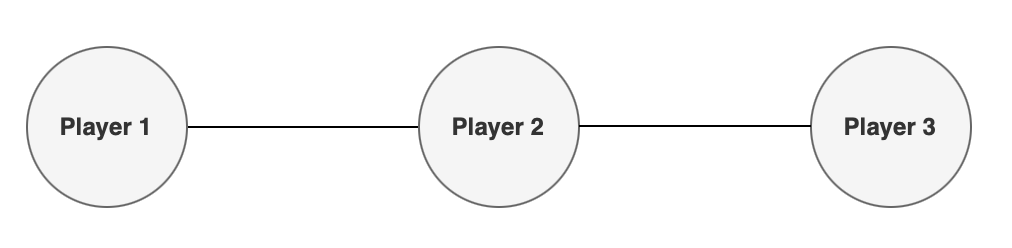
\includegraphics[width = 0.7\textwidth]{Figures/ThreePlayerNetwork.png}
    \caption{\label{fig::ThreePlayerNetwork}}
  \end{figure}

  As an adaptation, we take the example of a three player chain, as depicted in Figure \ref{fig::ThreePlayerNetwork}. In this example, we first assume that the network is simple (i.e. there are no self-loops and $w^{\mu \mu} = 0$). The aggregation matrix can be given as

  \begin{equation}
    W = \begin{bmatrix}
      0 & 1 & 0 \\
      w & 0 & 1 - w \\
      0 & 1 & 0
    \end{bmatrix}, \; w \in (0, 1).
  \end{equation}


  We first consider the zero-sum case to show that it does indeed converge to an equilibrium as expected. Note that the zero-sum condition given for the three player chain is given as

  \begin{equation}
    x \cdot A y + y \cdot B (w x + (1-w)z) + z \cdot C y = 0. \hspace{0.5cm} \forall x, y, z \in \Delta_1 \times \Delta_2 \times \Delta_3
  \end{equation}

  in which we use the notation that $x, y, z$ (resp. $A, B, C$) denote the strategies (resp. payoffs) of agents 1, 2 and 3 respectively. This condition is satisfied if we fix $B$ and choose

  \begin{align}
    A & = - w B^T \\
    C & = - (1 - w) B^T. 
  \end{align}

  As such in the following example, we will set $B = B_\beta$ with the choice $\beta \approx 0.576$ and set $A$ and $C$ according to the above with the choice $w \approx 0.288$. The orbits that these payoff matrices generate can be seen in Figure \ref{fig::convergentShapley}, in which, for each player, they converge to the Nash Equilibrium which, for each player, lies in the centre of the simplex.

  Let us now make the slight modification in the definition of C so that

  \begin{equation}
    C  = - (1 - w) B, 
  \end{equation}

  with no alteration to $A$. The modification itself is small, however it results in the zero-sum assumption being violated. With the same choices of $\beta$ and $w$, this results in the periodic orbit seen in Figure \ref{fig::nonconvergentShapley}. Here, the orbits reach a stable limit cycle which to be centred around the interior NE.

  \begin{figure}[t]
    \centering
    \begin{subfigure}[b]{0.4 \textwidth}
      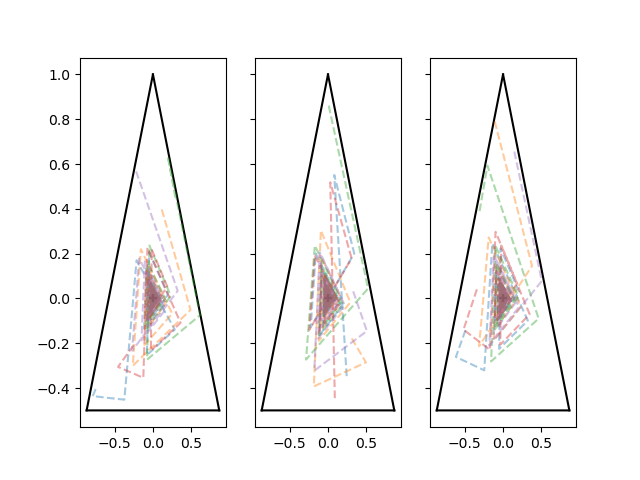
\includegraphics[width = \textwidth]{Figures/convergentShapley.png}
    \caption{\label{fig::convergentShapley}}
    \end{subfigure}
    \begin{subfigure}[b]{0.4 \textwidth}
      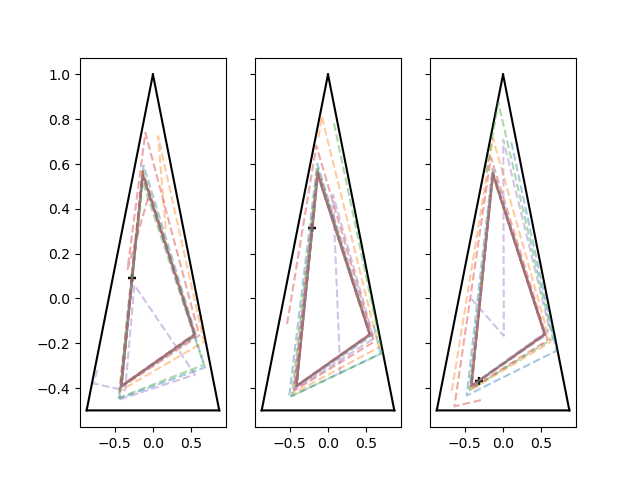
\includegraphics[width = \textwidth]{Figures/nonConvergentShapley.png}
      \caption{\label{fig::nonconvergentShapley}}
    \end{subfigure}
    \caption{\label{fig::Shapley}}
  \end{figure}


  \begin{figure}[t]
    \centering
    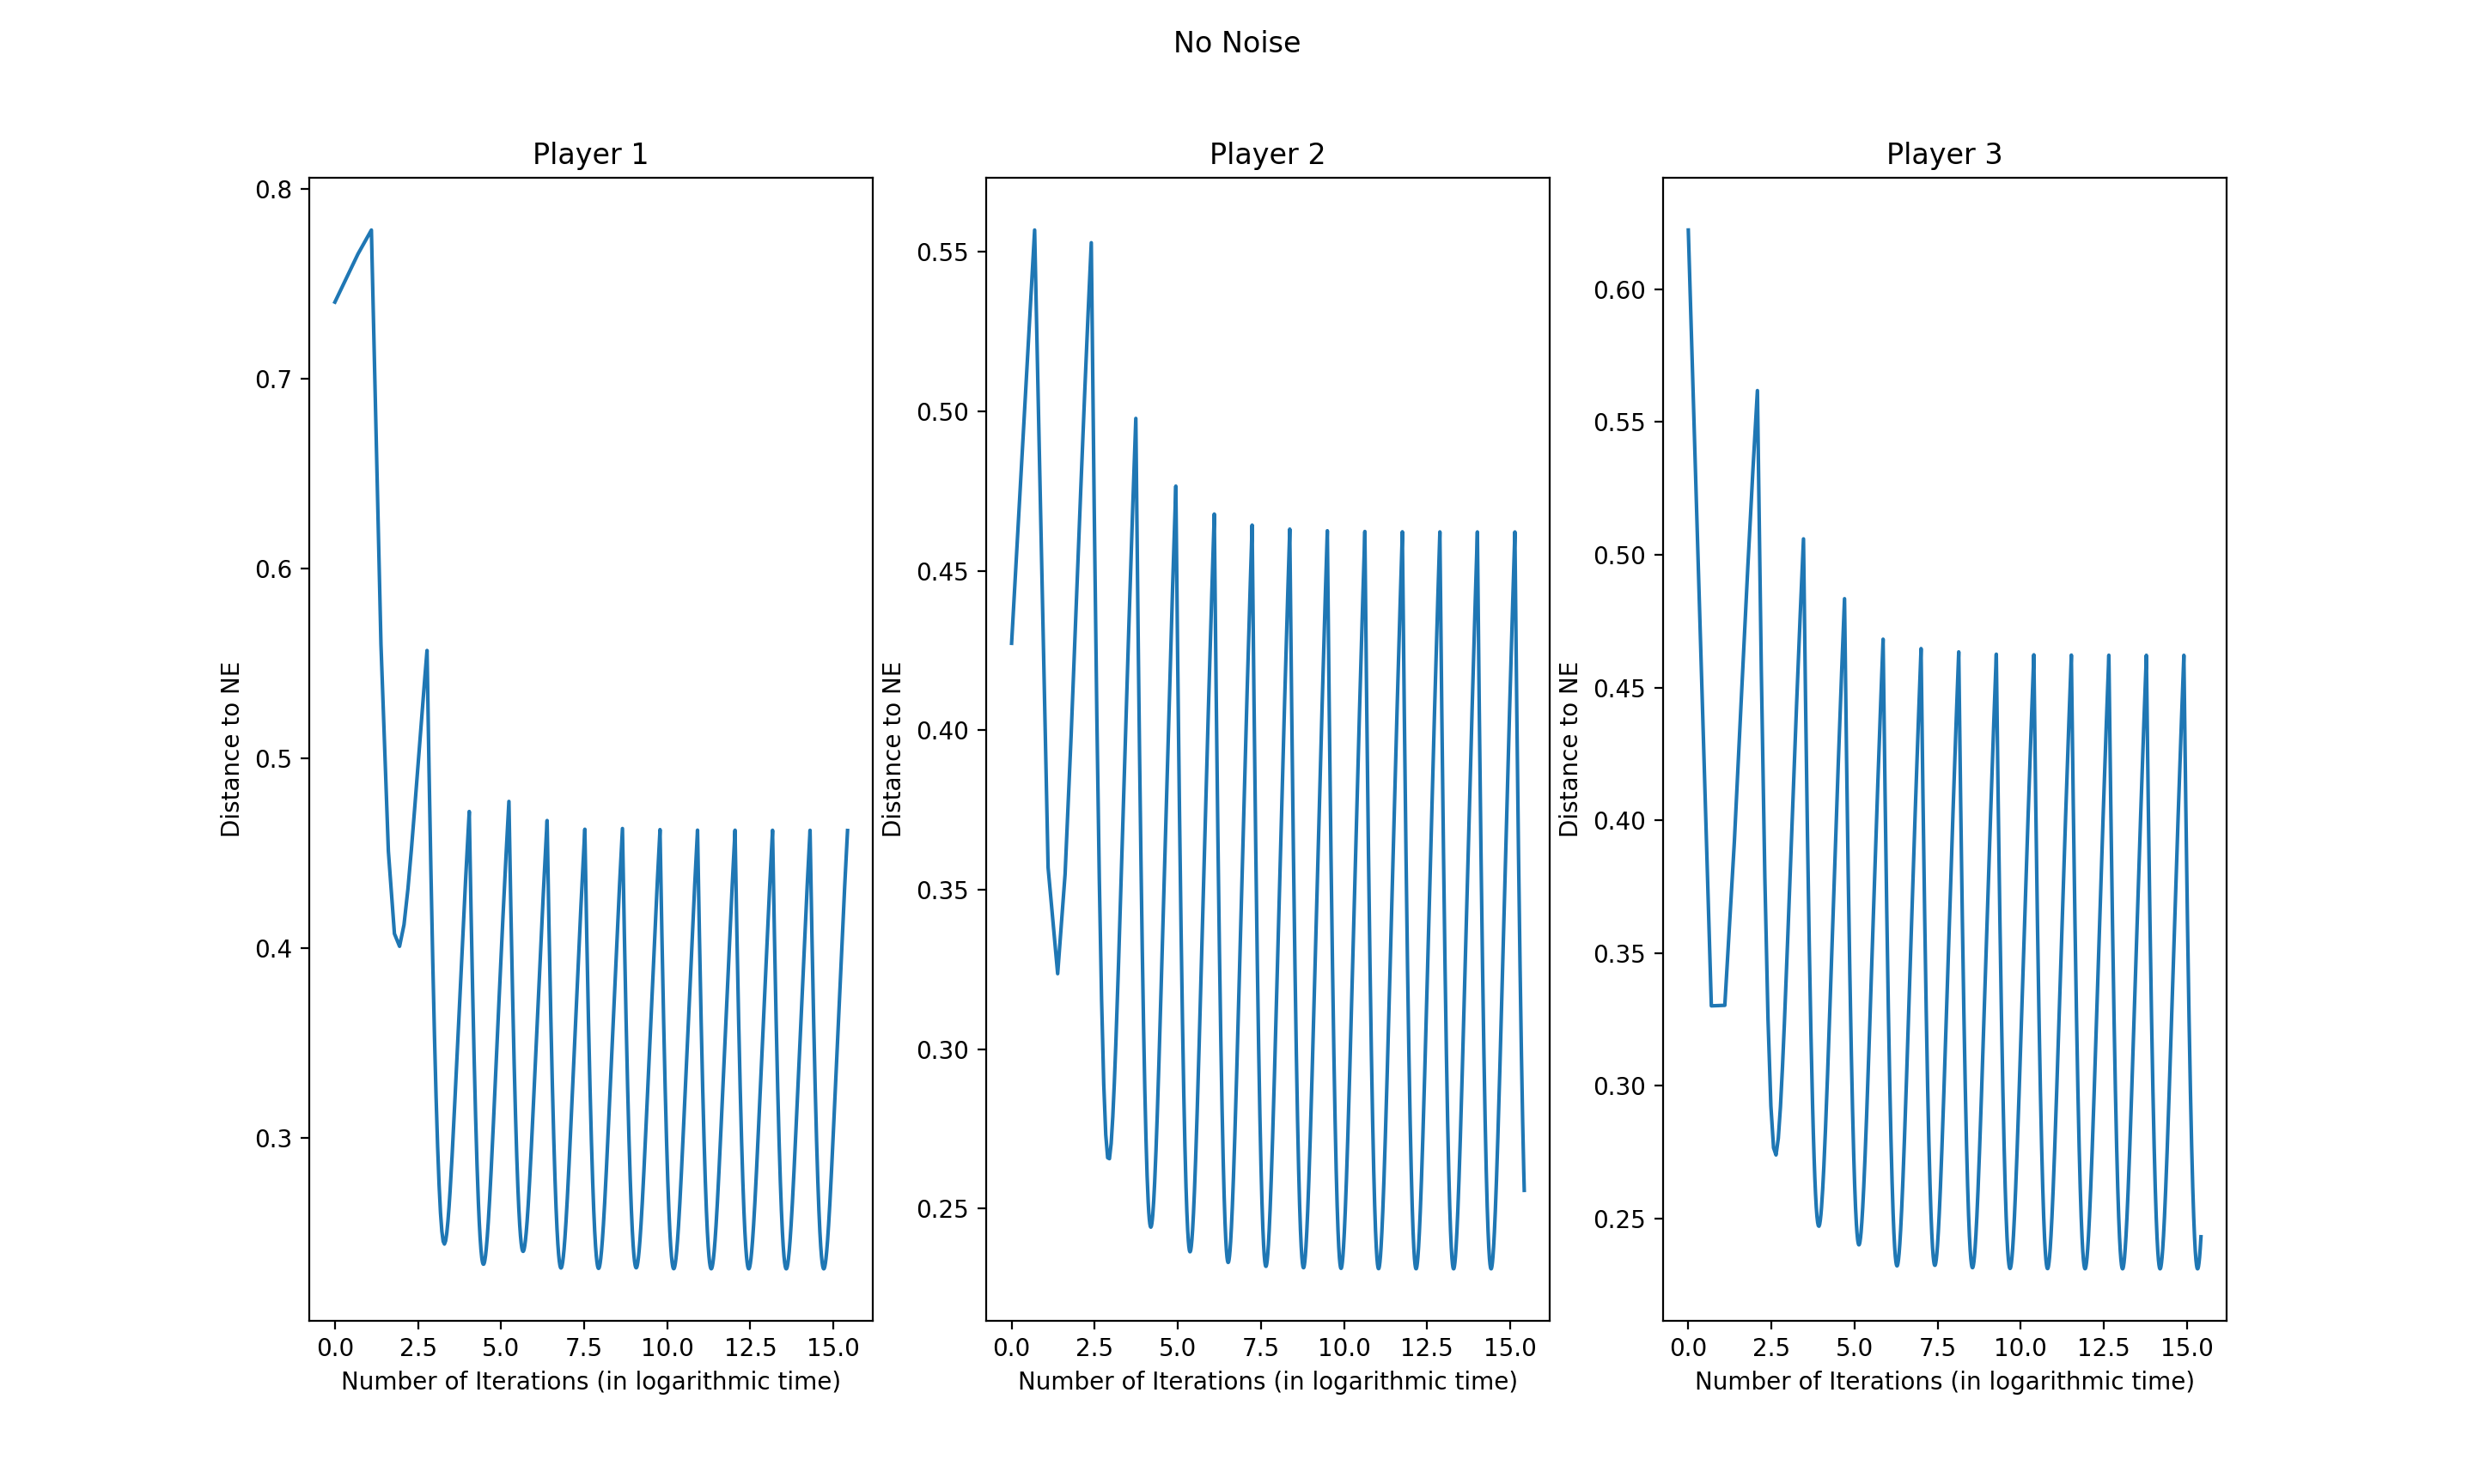
\includegraphics[width = 0.7 \textwidth]{Figures/3PlayerChainNoNoise.png}
    \caption{\label{fig::3PlayerChainNoNoise}}
  \end{figure}

  As such, we can see that convergent behaviour is not necessarily the norm in the NA-CTFP dynamics. In fact, for the family of games discussed above, we were unable to find non-periodic behaviour for any choice of $\beta$ strictly between 0.5 and 1 for any $w$ between 0.2 and 0.8 (so that the influence of player 1 and player 3 on player 2 is not negligible). This suggests that, far from being rare, in fact NA-CTFP lends itself to an incredibly rich variety of dynamics which can be explored as future work.
  

  \subsection{Addition of Noise}

  \begin{figure}[t]
    \centering
    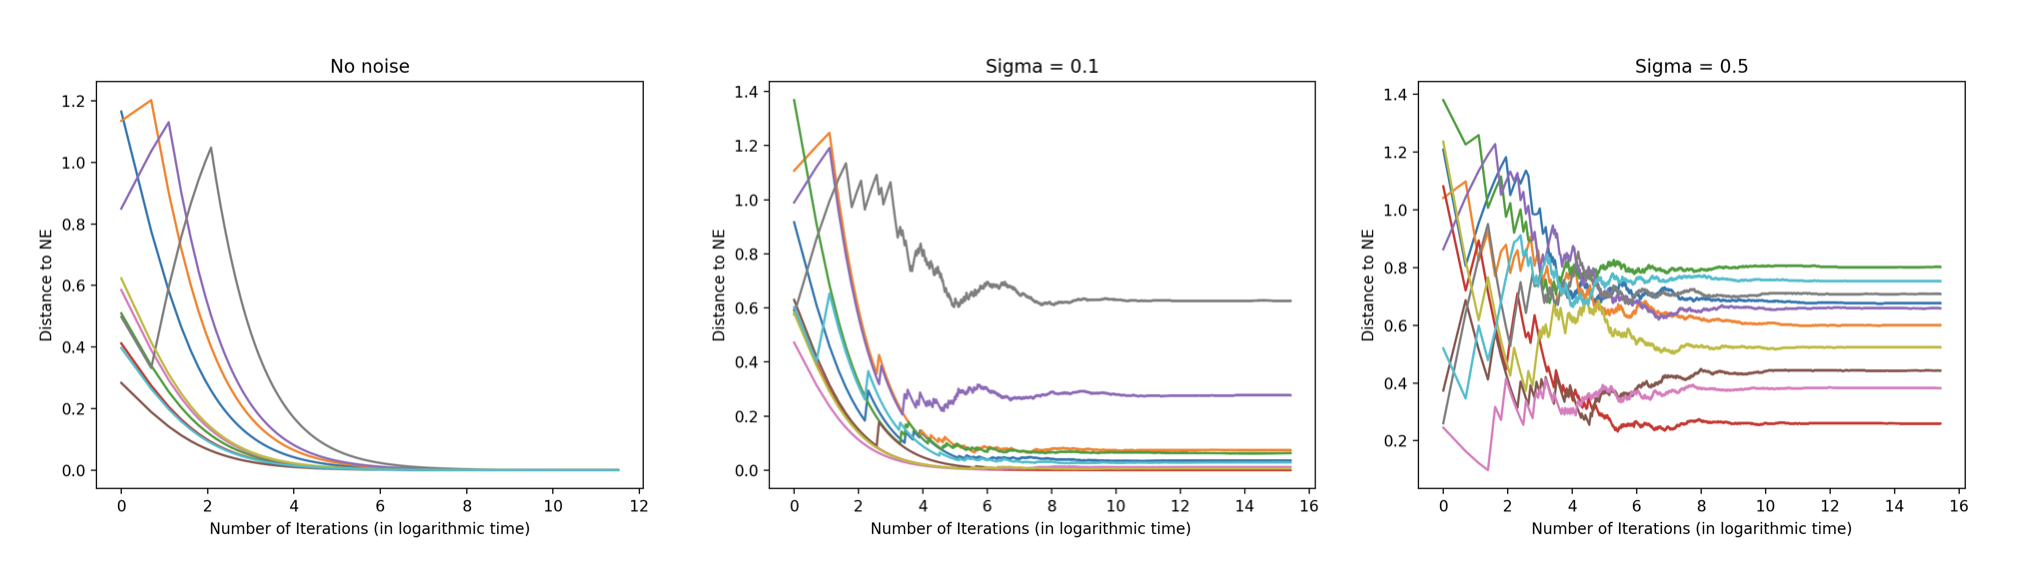
\includegraphics[width = \columnwidth]{Figures/Noise10Player.png}
    \caption{\label{fig::Noise10Player}}
  \end{figure}

  \begin{figure}[t]
    \centering
    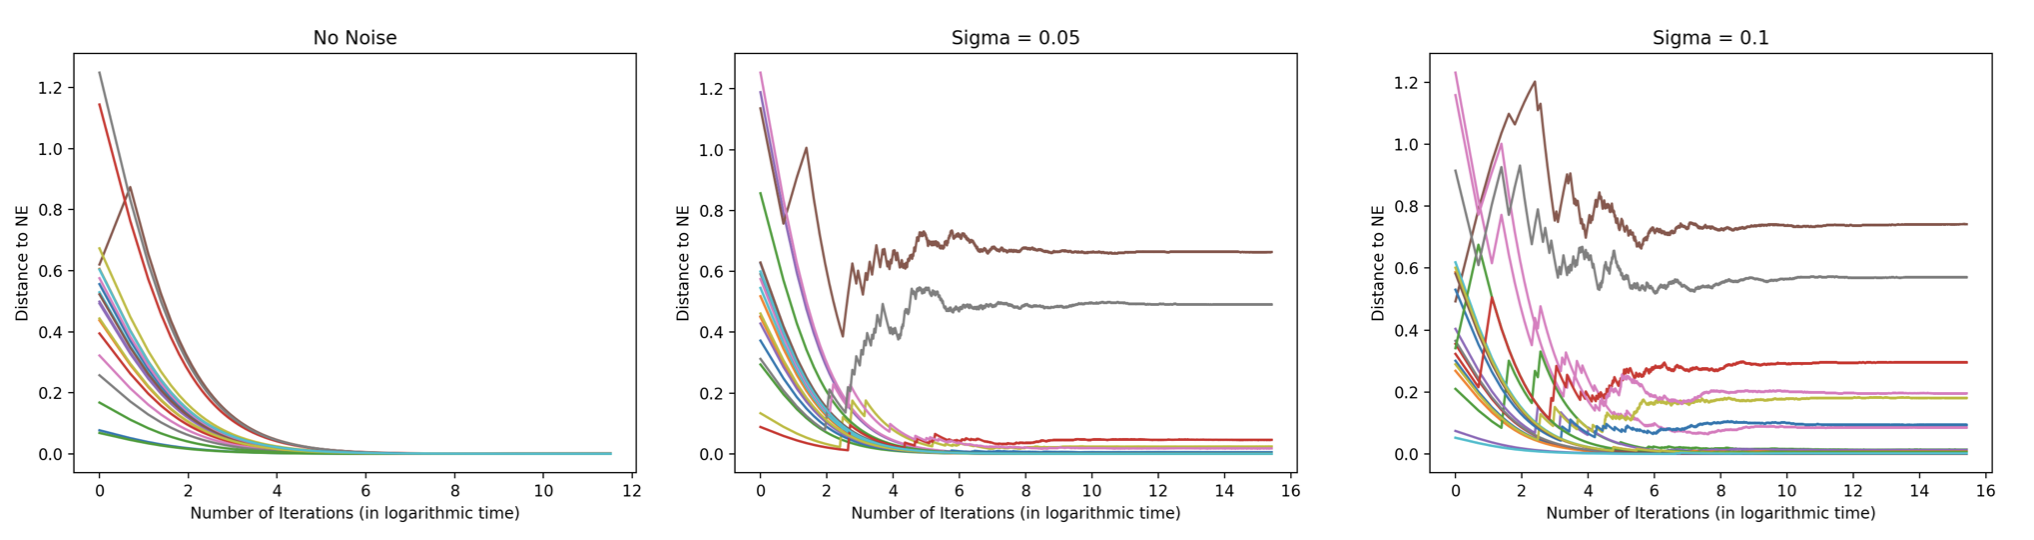
\includegraphics[width = \columnwidth]{Figures/Noise20Player.png}
    \caption{\label{fig::Noise20Player}}
  \end{figure}

  \begin{figure}[t]
    \centering
    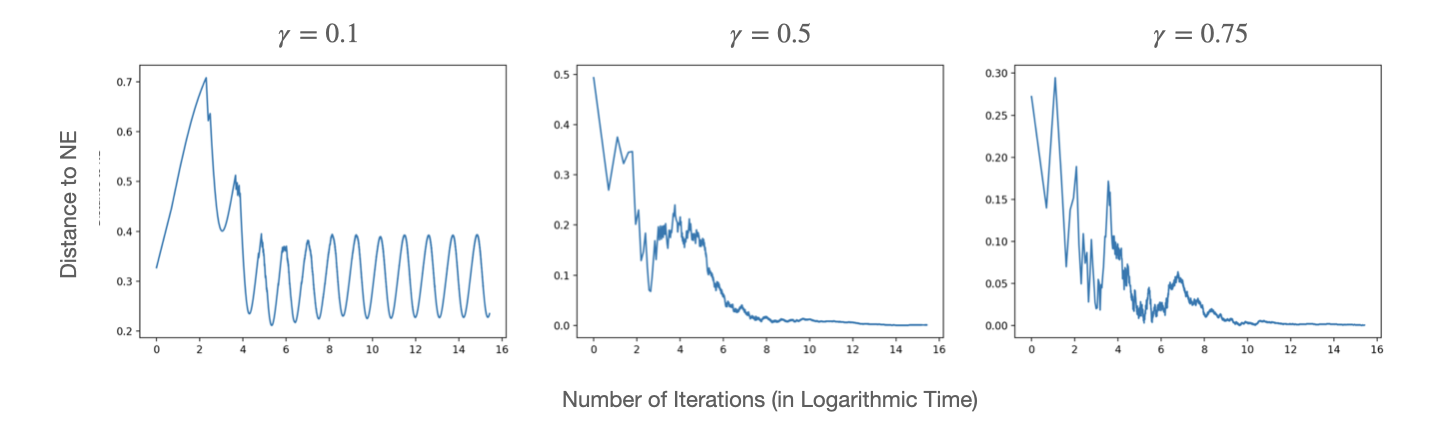
\includegraphics[width = \columnwidth]{Figures/3PlayerChainNoise.png}
    \caption{\label{fig::3PlayerChainNoise}}
  \end{figure}

  The fictitious play process in NA games requires that, at each time step, an agent takes a
  `measurement' of the aggregate strategy of its neighbours. It is on this measurement that they
  update their own strategy. It stands to reason then, that in real environments this measurement
  may be corrupted by noise. 
  
  As such, we investigate the effect that introducing additive noise has
  on CTFP in a zero-sum NA game. We do this in the following manner: at each time step, the
  reference signal $\refmu(t)$ is adjusted to $\refmu + \gamma \xi$ where $\xi$ is drawn from the
  standard normal distribution (zero mean and unit variance). By varying $\gamma$, we vary the
  strength of the noise. We vary $\gamma$ up to $0.5$ since, above this value, noisy measurements
  are likely to lie outside of the simplex. Since $\refmu$ is constrained to lie within $\Delta$, we
  can consider the range $\gamma \in [0, 0.5]$ to be the \emph{physical region}, in which noise is meaningful.

  In Figure \ref{fig::Noise10Player}, we consider a zero-sum NA game with 10 players. When there is
  no noise, it can be seen that FP reaches a fixed point which, since we set $w^{\mu \mu} = 0$,
  corresponds to an NE. After increasing $\gamma$, however, we find that the agents no longer
  converge to this NE, but rather shift away from it. What is interesting, however, is that the
  orbits do still reach a stationary state in the long run which suggests that FP is still able to
  converge with the introduction of noise. Figure \ref{fig::Noise20Player} shows similar behaviour
  for $N = 20$, and in our experiments we found this to be ubiquitous regardless of the choice of
  $N$ or $n$. 

  In Figure \ref{fig::3PlayerChainNoise} we revisit the Three Player Chain of Section
  \ref{sec::NonConv}, now under the influence of additive noise. For the sake of brevity, we only
  display the distance to the Nash Equilibrium of the first player's action, since the other agents
  behave in the same way. It can be seen that a small amount of noise has the effect of decreasing
  the size of the periodic orbit (c.f. Figure \ref{fig::3PlayerChainNoNoise}). However, as $\gamma$
  is increased to $0.5$, the algorithm seems to exhibit convergence to the NE. The implication is
  that the addition of noise may cause periodic behaviour to break and lead to the Nash Equilibrium.
  An interesting point to note is that this behaviour is in stark contrast to the replicator
  dynamic (RD) \cite{Maynard-Smith}, another adaptive algorithm linked to multi agent learning
  \cite{CyclesAdversarialLearning}. In \cite{Imhof} and \cite{Galla}, it was found that the
  introduction of random mutations can remove convergent behaviour and instead lead to periodicity. 
  
\section{Concluding remarks}


\section*{Broader Impact}

Authors are required to include a statement of the broader impact of their work, including its ethical aspects and future societal consequences. 
Authors should discuss both positive and negative outcomes, if any. For instance, authors should discuss a) 
who may benefit from this research, b) who may be put at disadvantage from this research, c) what are the consequences of failure of the system, and d) whether the task/method leverages
biases in the data. If authors believe this is not applicable to them, authors can simply state this.

Use unnumbered first level headings for this section, which should go at the end of the paper. {\bf Note that this section does not count towards the eight pages of content that are allowed.}

\begin{ack}
Use unnumbered first level headings for the acknowledgments. All acknowledgments
go at the end of the paper before the list of references. Moreover, you are required to declare 
funding (financial activities supporting the submitted work) and competing interests (related financial activities outside the submitted work). 
More information about this disclosure can be found at: \url{https://neurips.cc/Conferences/2020/PaperInformation/FundingDisclosure}.


Do {\bf not} include this section in the anonymized submission, only in the final paper. You can use the \texttt{ack} environment provided in the style file to autmoatically hide this section in the anonymized submission.
\end{ack}

\section*{References}

References follow the acknowledgments. Use unnumbered first-level heading for
the references. Any choice of citation style is acceptable as long as you are
consistent. It is permissible to reduce the font size to \verb+small+ (9 point)
when listing the references.
{\bf Note that the Reference section does not count towards the eight pages of content that are allowed.}
\medskip

\small

[1] Alexander, J.A.\ \& Mozer, M.C.\ (1995) Template-based algorithms for
connectionist rule extraction. In G.\ Tesauro, D.S.\ Touretzky and T.K.\ Leen
(eds.), {\it Advances in Neural Information Processing Systems 7},
pp.\ 609--616. Cambridge, MA: MIT Press.

[2] Bower, J.M.\ \& Beeman, D.\ (1995) {\it The Book of GENESIS: Exploring
  Realistic Neural Models with the GEneral NEural SImulation System.}  New York:
TELOS/Springer--Verlag.

[3] Hasselmo, M.E., Schnell, E.\ \& Barkai, E.\ (1995) Dynamics of learning and
recall at excitatory recurrent synapses and cholinergic modulation in rat
hippocampal region CA3. {\it Journal of Neuroscience} {\bf 15}(7):5249-5262.

\end{document}
